\chapter{Heart rate sensor}\label{ch:heartRate}
%**********************************************

%**********************************************
\section{Introduction} \label{sec:heartIntro}
%**********************************************
% What to introduce:\newline 
% Explain what parameters you need to design the Sallen Key for.\newline
% Explain what parameters you need to design the Passive filter. \newline
% Explain the sources cited for the comparator design and the time of the pulses. \newline
In this chapter, the design for the Sallen \& Key HPF, Passive LPF and Comparator will be explained and what sources where consulted in the designed process.\par
The Sallen \& Key HPF design \cite{Sallen} can be used to not only filter the signal above a desired frequency, but by adding a resistor feedback the signal can also be amplified. Amplification reduces the quality of the signal ($Q$), thus the amplification must not be too large . This method is used in the design to make it easier for thresholding in a later stage. In order to minimise design expenses, the LPF design is based on a passive filter \cite{LPF}. A single order filter does enough to filter excess noise to a degree, but in order to smooth out the signal further, a second phase is added to the design to create a second order passive LPF. 


% Introduce the reader to what you want to present in this chapter. 
% Include any references to literature you feel is needed. 
% In this section, you put a very short summary of infrormation you gatherered from literature (papers, web sites, datasheets) that you used to do the design. Be sure to include the references, which you can add in the \texttt{References.bib} file. 
% Rather than just copy\&pasting \footnote{I have a little bee in my bonnet about people who say ``cut\&paste'' - if it were cut, it would not be there anymore!} from the datasheet, give your own circuit diagrams. Remember, it is important that someone who reads your report must be able to reproduce your results. 

% Some examples of how to cite (all in \texttt{References.bib}): 
% It was stated by \cite{Booysen:2013} that ... . Subsequently, he changed his mind and said in  \cite{Gerber:2019} that ... .
% While \cite{WebsiteOpAmp} claims it to be ... .


%**********************************************
\section{Design} \label{sec:heartDesign}
%**********************************************
Before designing the filter, the frequency response must first be inspected to determine which frequencies are desired and which are not. In Fig \ref{fig:FFT} a \SI{150}{BPM} heart beat is drawn in LTSpice using its built in FFT function, and shows 3 prominent frequencies between \SI{0.8}{\hertz} and \SI{4}{\hertz} and numerous spikes above \SI{10}{\hertz}. From this it can be concluded that the frequencies from \numrange{0.8}{4} \si{\hertz} is desired signal while anything above or below this range is noise.\par

\begin{figure}[H]
    \centering
    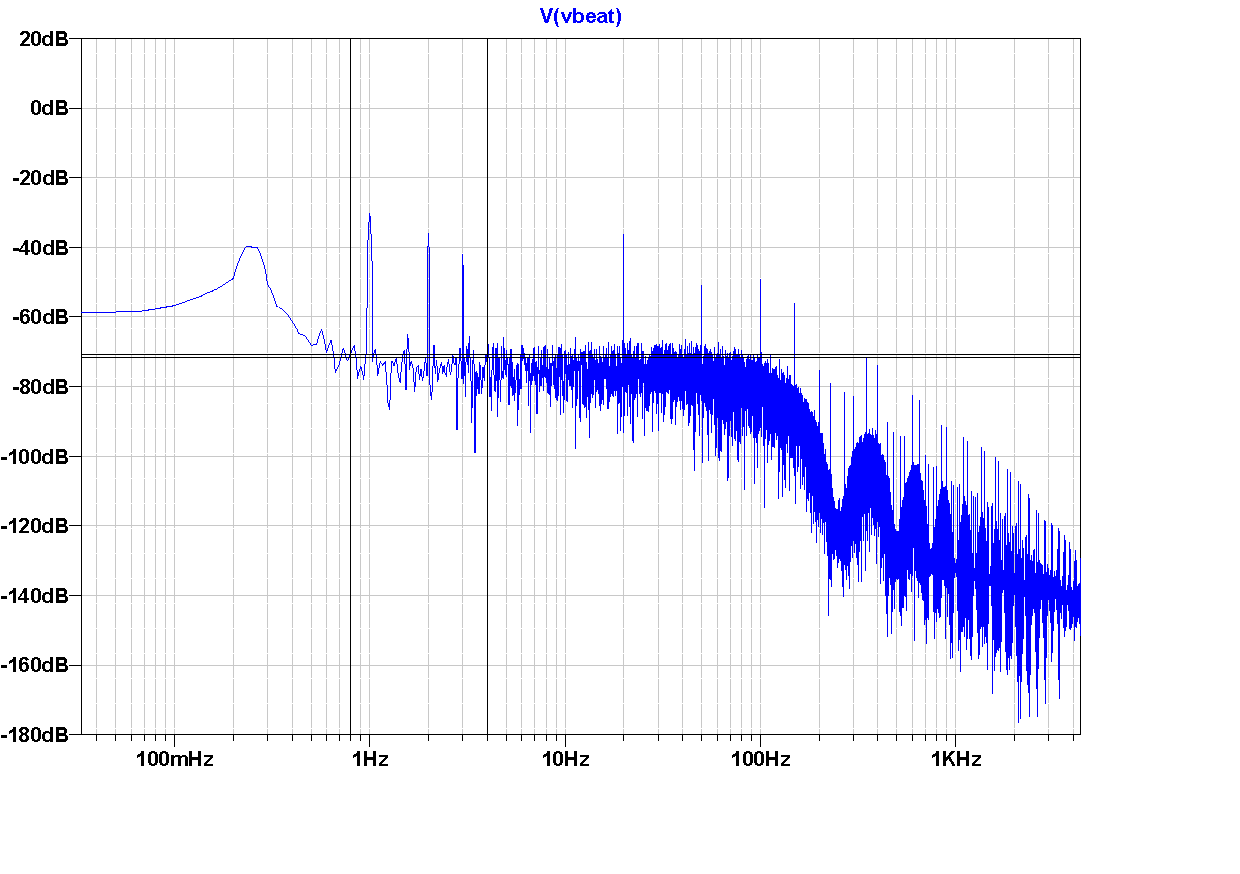
\includegraphics[width = 0.65\linewidth]{./Figures/FFT150BPM_cropped.pdf}
    \caption[Frequency response of Heartbeat]{FFT of a 150BPM Heart Beat Signal}
    \label{fig:FFT}
\end{figure}



 The HPF will thus be designed to suppress all frequencies below \SI{0.8}{\hertz}. The design layout will look like Fig. \ref{subfig:Sallen}. The HPF will be designed for a corner frequency ($f_{c}$) of \SI{0.8}{\hertz}. One can assume $R_{1} = R_{2} = R$ and $C_{1} = C_{2} = C$, then Eq. \ref{eq:HPFCorner} becomes Ep. \ref{eq:HPFCornerNew}. Using a standard capacitor value of \SI{1.5}{\micro\farad} for $C$, a resistor value can be approximated.
 
\begin{equation}
   f_{c} = \frac{1}{2 \pi \sqrt{R_{1} R_{2} C_{1} C_{2}}}
   \label{eq:HPFCorner} 
\end{equation} 

 \begin{equation}
    f_{c} = \frac{1}{2 \pi R C}  
    \label{eq:HPFCornerNew} 
\end{equation}

\[   R = \frac{1}{2 \pi f_{c} C} = \frac{1}{2 \pi \times 0.8 \times 1.5 \si{\micro}} = \SI{132629}{\Omega} \approx \SI{130}{\kilo\Omega}  \]
\par
To finish off the design of the HPF, the amplification factor must be designed. As noted in \cite{Sallen} the amplification is dependant on the quality factor, $Q$, which determines the amplification. Designing for a moderate quality factor of 3 gives the amplification and resistor values for $R_{3}$ and $R_{4}$ as follows in Eq. \ref{eq:AmpFactor} and Eq. \ref{eq:ResistorValuesHPF}. Assume $R_{4} = \SI{200}{\kilo\Omega}$.

\begin{equation}
    A = \frac{3 Q - 1}{Q} = \frac{3 (3) - 1}{3} = 2.66667  
    \label{eq:AmpFactor} 
\end{equation}
\[      A = 1 + \frac{R_{4}}{R_{3}} \implies  \frac{R_{4}}{R_{3}} = 1.66667    \]
\begin{equation}
    R_{3} = \frac{R_{4}}{1.66667} = \SI{119.9998}{\kilo\Omega} \approx \SI{120}{\kilo\Omega}
    \label{eq:ResistorValuesHPF} 
\end{equation}
 
 
 \begin{figure}
    \centering
    \begin{subfigure}[]{0.55\textwidth}
        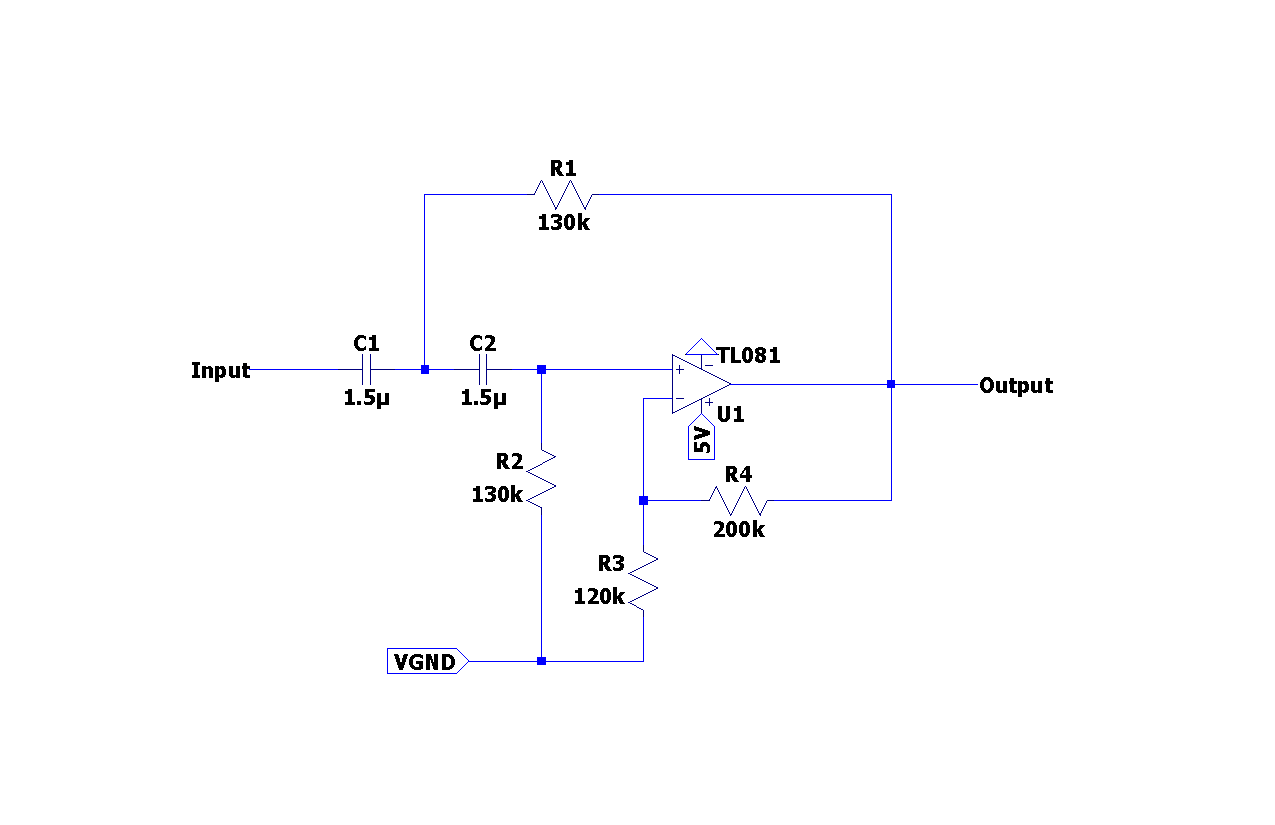
\includegraphics[width=\linewidth]{./Figures/HPFCircuit_cropped.pdf}
        \caption{Sallen \& Key HPF circuit diagram}
	    \label{subfig:Sallen}	
   \end{subfigure}
   \begin{subfigure}[]{0.35\textwidth}
        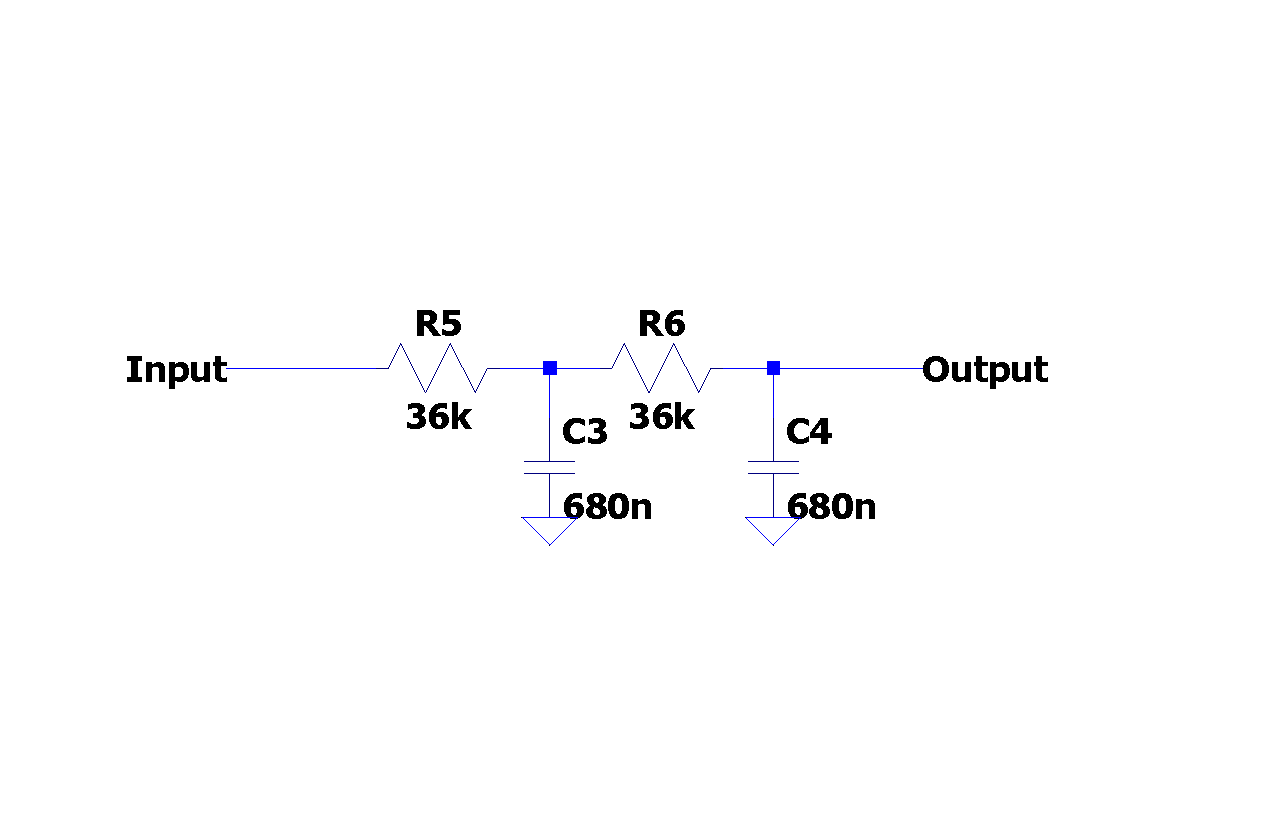
\includegraphics[width=\linewidth]{./Figures/LPFCircuit_cropped.pdf}
        \caption{Passive LPF circuit diagram}
	    \label{subfig:LPF}	
   \end{subfigure}
    \caption[Filters Circuit Diagrams]{Circuit Diagrams of a Sallen \& Key HPF and Passive LPF}
    \label{fig:CirDiagram}
\end{figure}
 
\par

The LPF will be designed to suppress all frequencies above \SI{4}{\hertz}. The design layout will look like Fig. \ref{subfig:LPF}. A second order passive LPF has to be designed for a different cutoff frequency than a normal first order LPF, which is usually the \SI{3}{\deci\bel} point. Using \cite{LPF} as reference, the new cutoff frequency is derived from Eq. \ref{eq:3dBFreq} where $n$ is the order of the filter and the \SI{3}{\deci\bel} point is \SI{4}{\hertz}. 
Now the resistor values for the LPF can be designed using \ref{eq:LPFCutoffFreq}, assuming that $R_{5}=R_{6}=R$ and $C_{3}=C_{4}=C=\SI{680}{\nano\farad}$. 

\begin{equation}
    f_{(\SI{-3}{\deci\bel})} = f_{C} \sqrt{2^{(\frac{1}{n})}-1}
    \label{eq:3dBFreq}
\end{equation}
\[      f_{C} = \frac{f_{(\SI{-3}{\deci\bel})}}{f_{(\SI{-3}{\deci\bel})}}  =   \frac{\SI{4}{\hertz}}{\sqrt{2^{(\frac{1}{2})}-1}} = \SI{6.215}{\hertz} \]
\begin{equation}
    f_{C} = \frac{1}{2 \pi \sqrt{R_{5}R_{6}C_{3}C_{4}}} = \frac{1}{2\pi R C}
    \label{eq:LPFCutoffFreq}
\end{equation}
\[      R = \frac{1}{2 \pi f_{c} C} = \frac{1}{2 \pi \times 6.215 \times 680 \si{\nano}} = \SI{37.66}{\kilo\Omega} \approx \SI{36}{\kilo\Omega}  \]\par

A simple comparator design, seen in Fig. \ref{fig:Comparator}, that only uses an op-amp will be used to push the signal from \numrange{0}{5} \si{\volt}. The threshold value is determined by $R_{7}$ and $R_{8}$. As the signal through the HPF is already centred around \SI{2.5}{\volt}, any deviation in the DC component of the signal is neglected. Assuming the filtered response of a heartbeat will approximate a sawtooth signal centred around \SI{2.5}{\volt}, the comparator must be designed for the highest frequency as it will have the shortest pulse. A 150BPM signal will subsequently have a period of \SI{400}{\milli\second}. For simplicity, the thresholding can be designed for \SI{200}{\milli\second}, or approximately \SI{2.5}{\volt}. To achieve this, $R_{7}$ and $R_{8}$ must be equal. The thresholding should be large enough to allow for a deviation of $\pm\SI{10}{\milli\volt}$ in amplitude, while also eliminating the need for a One Shot component. The resistors must also be large to limit current draw. Thus $R_{7}=R_{8}=330k$.\par
Regarding op-amps, the HPF handles a small input voltage with a relatively small swing. For this stage, the opamp will never reach the \numrange{0}{5} \si{\volt} rails, and can therefore use a TL081 op-amp \cite{TL081}. The comparator however, will receive an larger, amplified signal and will need to push the voltage between the \SI{5}{\volt} and \SI{0}{\volt} rails, therefore needing a much stronger op-amp, such as the TLC2272 op-amp \cite{TLC2272}.

\begin{figure}[H]
    \centering
    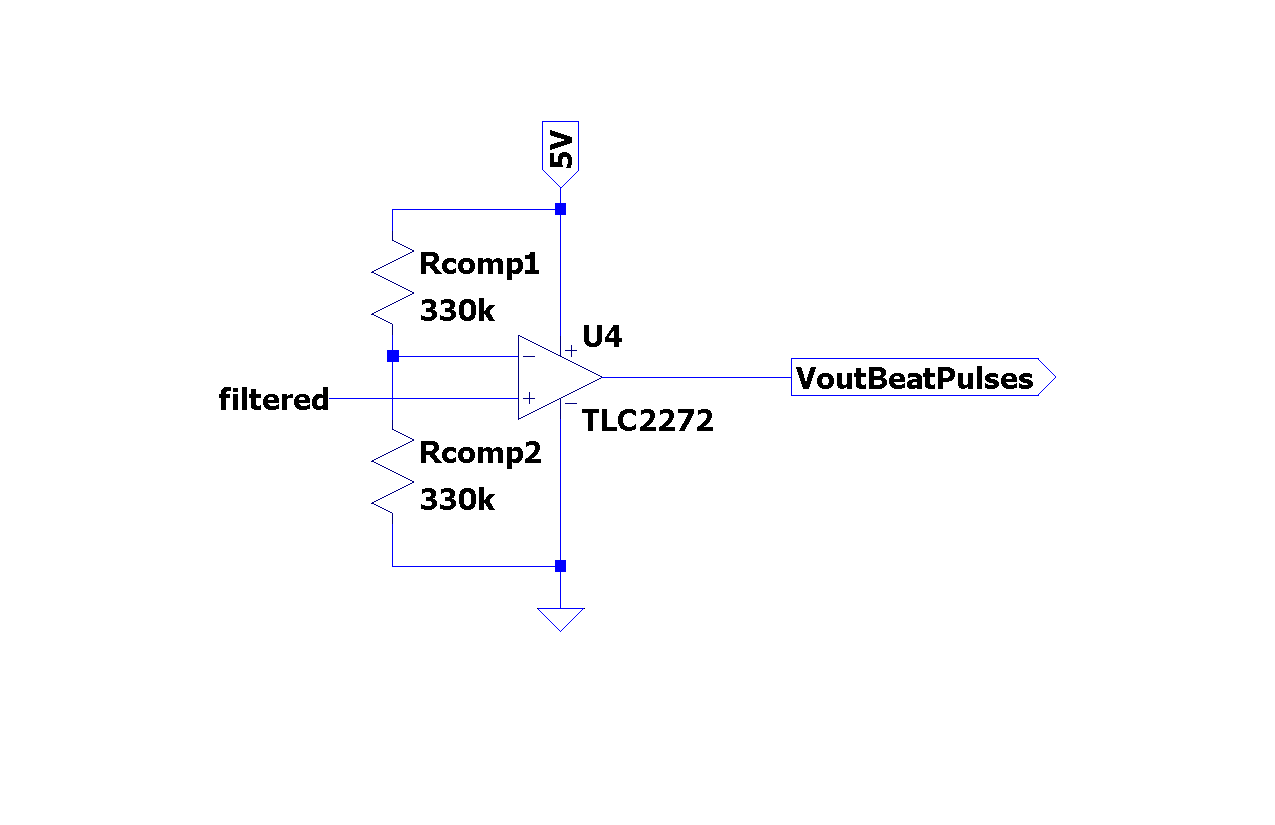
\includegraphics[width = 0.4\linewidth]{./Figures/CompCircuit_cropped.pdf}
    \caption[Comparator Circuit Diagram]{Op-amp comparator circuit}
    \label{fig:Comparator}
\end{figure}

% In this section, you need to capture your design, which should include the following: 
% \begin{itemize}
%   \item Design rationale, i.e. what your thinking was behind the design. For example, explain that you had to first analyse the heart beat signals before you could design the filtering. 
%   \item References to literature/sources as appropriate \cite{WebsiteOpAmp}.  
%   \item You can assume the reader has an E\&E degree, and will not need detail explanations of trivial information (e.g. what a resistor is, or what Ohm's law is).  
%   \item Design calculations, for example to determine resistor values and capacitor values, or to check for allowed voltage and current ranges and levels. These calculations should also give expected outputs, which hopefully matches the simulated values. Importantly, they are based on maths, and not on simulation - there is a difference. 
%   \item Analysis of given or expected input conditions. 
%   \item Expected values and ranges based on your design. 
%   \item Explain your choice of supply buy referring to the advantages and disadvantages of each. 
%   \item Circuit diagram like the one in Figure \ref{fig:circuit_diagram}. I used ``print to PDF'' from LTSpice,  but feel free to use a cropped screengrab if you are PDF-challenged and do not have a PDF printer (there are some free PDF creators online). Also have a look at the demo video on SUNLearn. 
% \end{itemize}

% For your benefit, here is how to write values with units: $\SI{150}{\milli\Omega}$ or \SI{199}{myUnits}, and this is how we write ranges: \numrange{2}{5} \si{\kilo\volt}.

% Here is an inline equation $ \frac{55}{45+3}$. Here is a numbered equation in Eq. \ref{eq:myNumberedEquation}.
% \begin{equation}
%   a = \frac{55}{45+3}
%   \label{eq:myNumberedEquation}. 
% \end{equation}. 



% \begin{figure}
%  \footnotesize
%   \centering
%   \begin{subfigure}[]{0.45\textwidth}
%         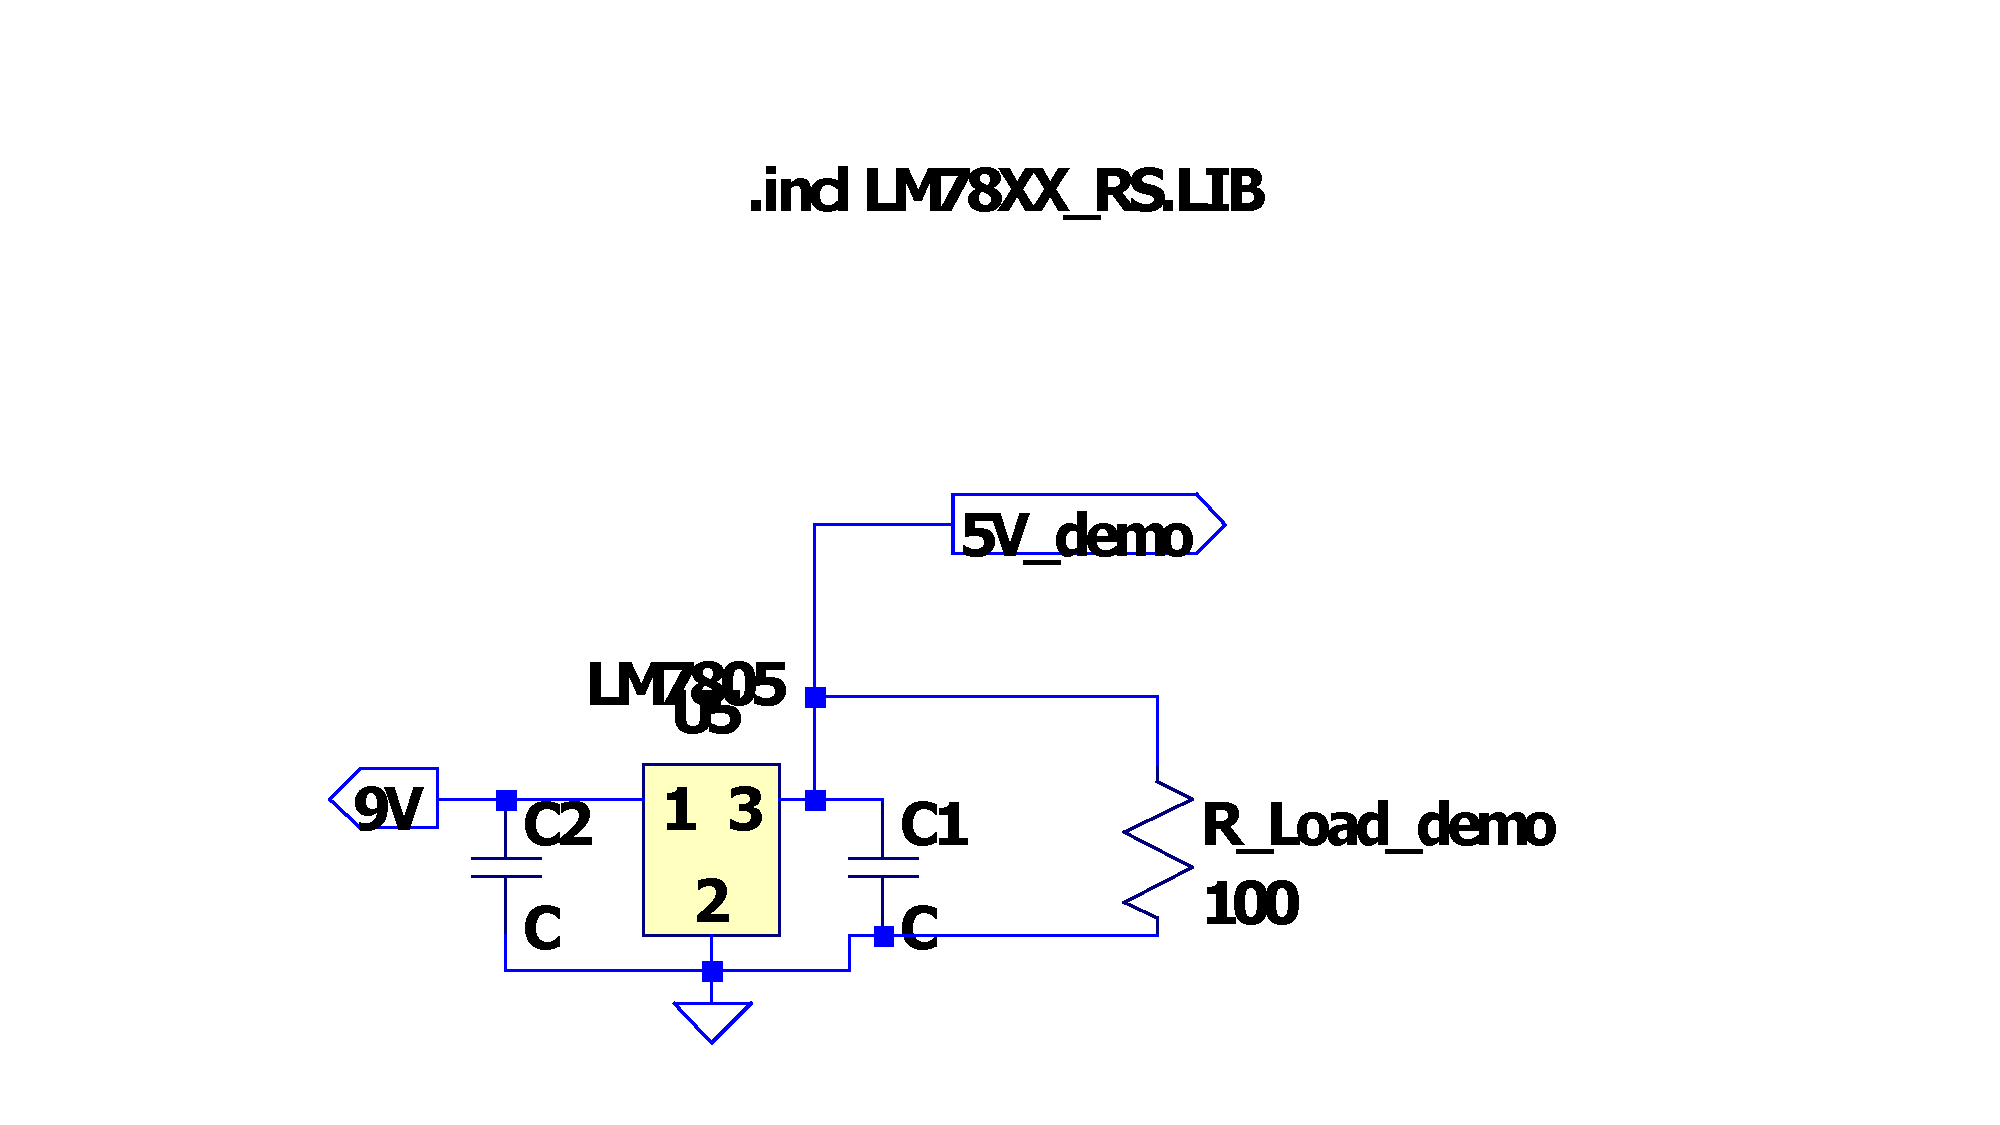
\includegraphics[width=\linewidth]{./Figures/E344_Ass1VoltRegulator_cct}
% 	  \caption{Linear voltage regulator.} \label{subfig:linear_circuit_diagram}	
%   \end{subfigure}
%   \begin{subfigure}[]{0.45\textwidth}
%   	 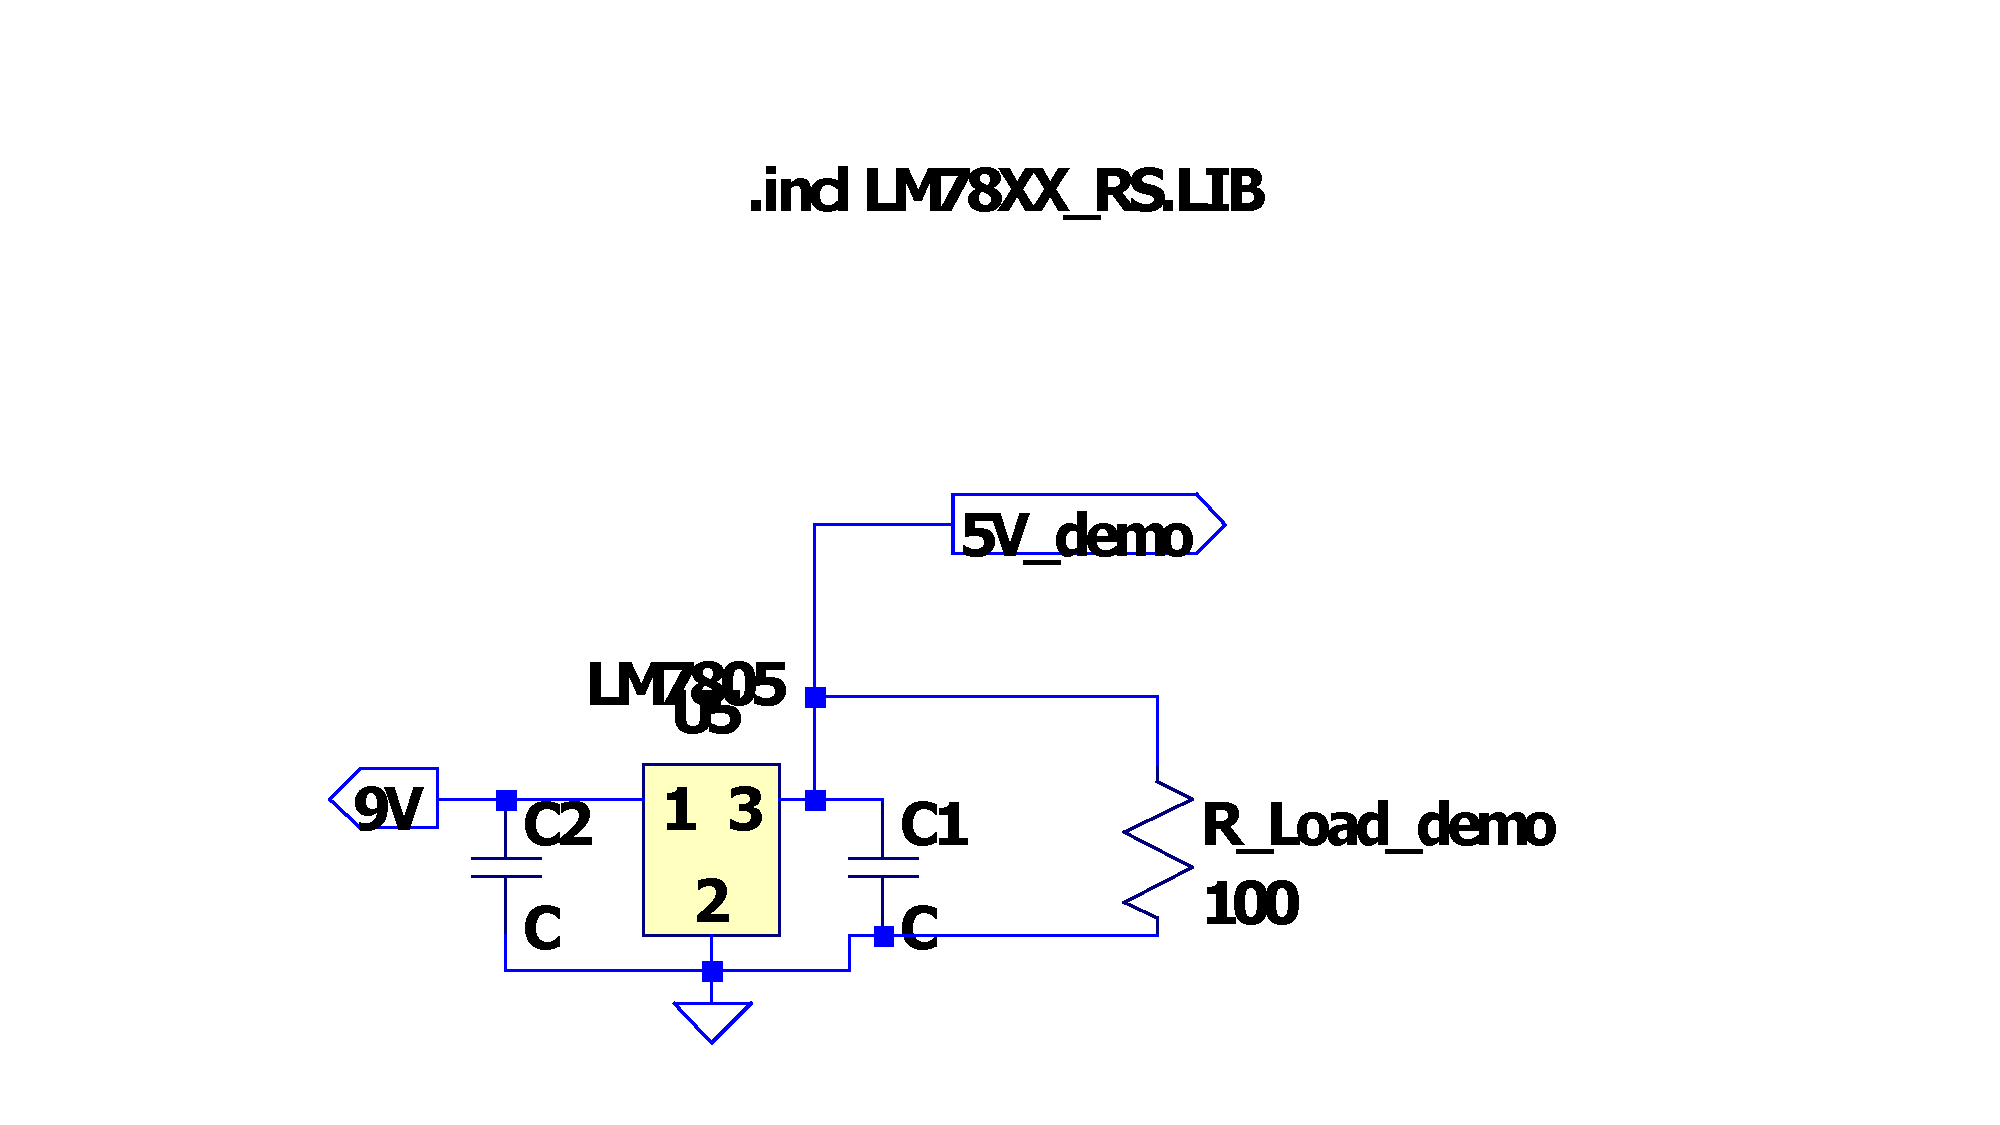
\includegraphics[width=\linewidth]{./Figures/E344_Ass1VoltRegulator_cct}
% 	  \caption{Switchmode voltage regulator.} \label{subfig:switchmode_circuit_diagram}	
%   \end{subfigure}
%   \begin{subfigure}[]{0.95\textwidth}
%   	 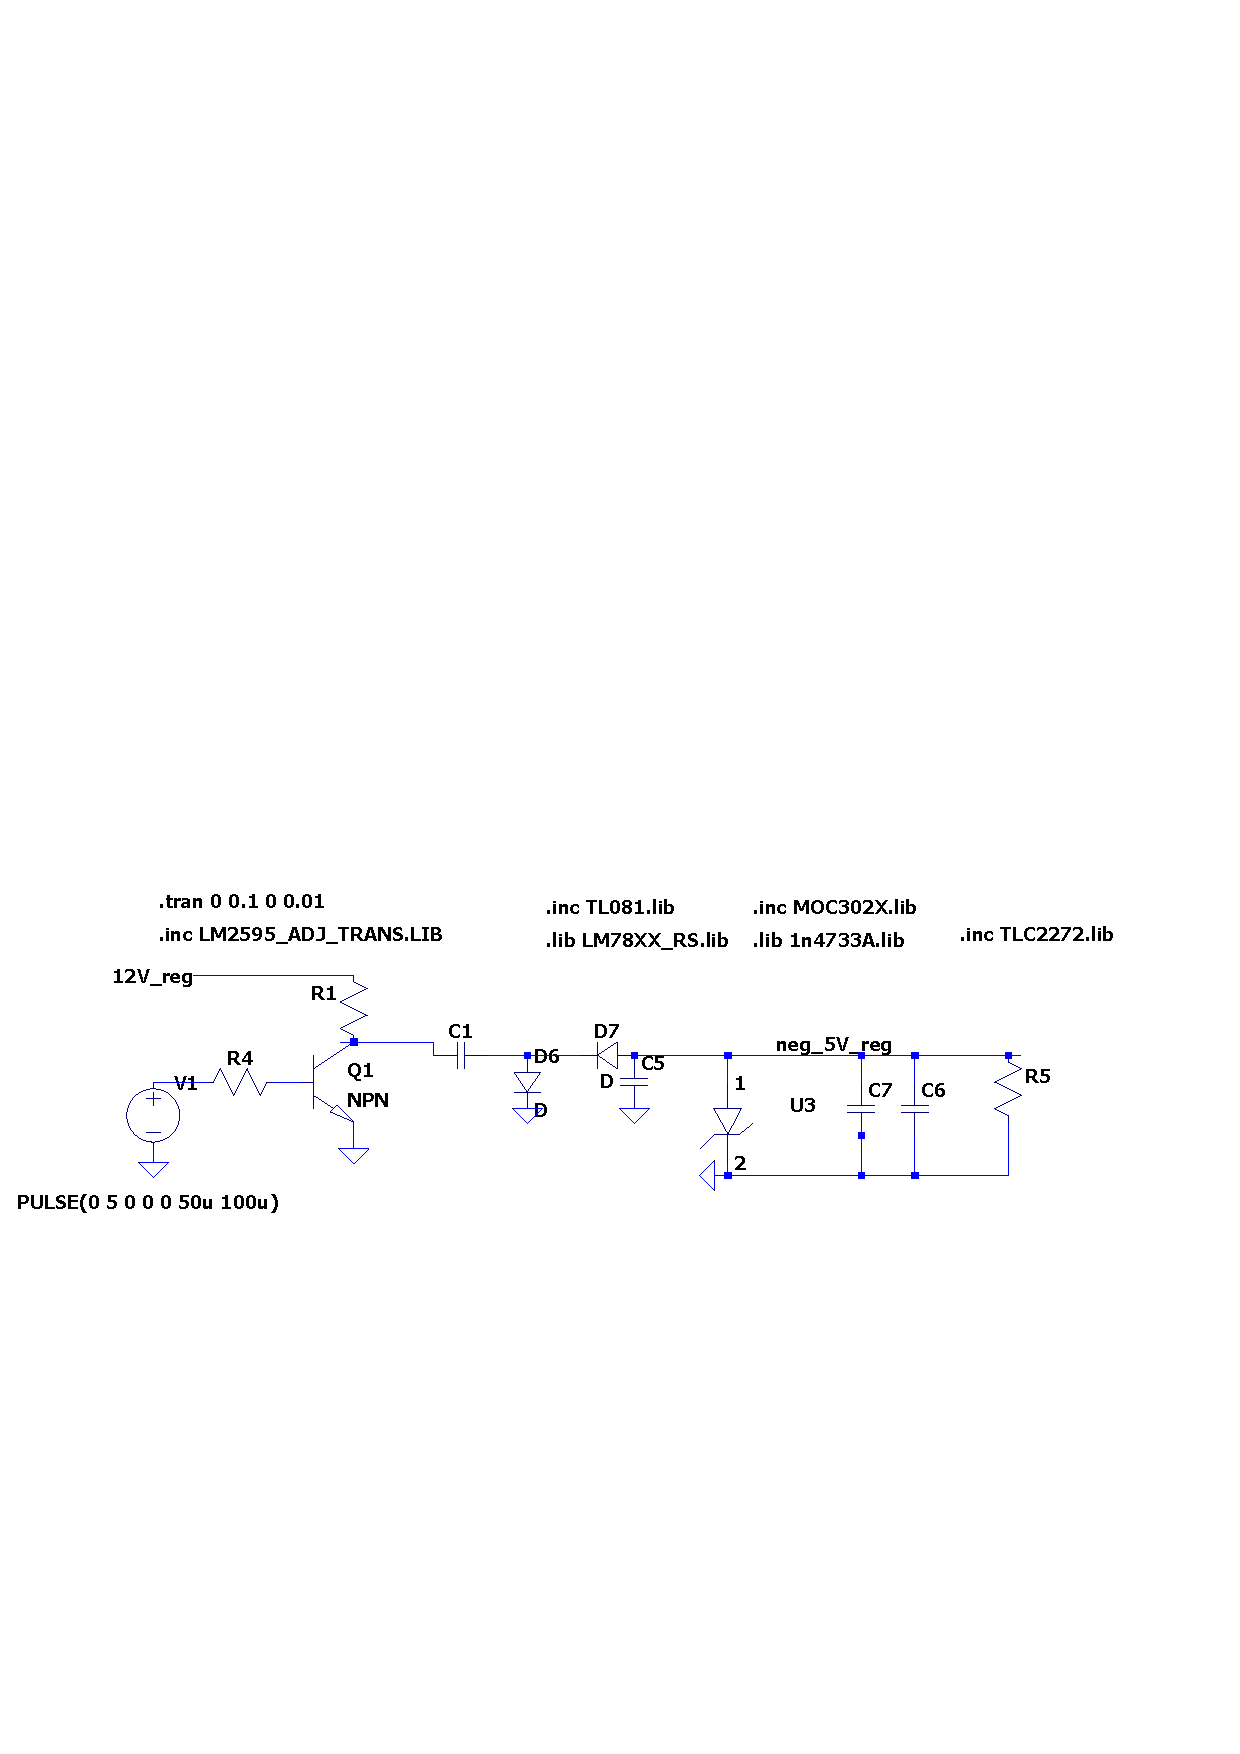
\includegraphics[width=\linewidth]{./Figures/CctDia}
% 	  \caption{Chargepump voltage regulator.} \label{subfig:chargepump_circuit_diagram}	
%   \end{subfigure}
   
%   \caption {Circuit diagrams of the two voltage regulators, and another irrelevant one}.

%       \label{fig:circuit_diagram}
%  \end{figure}
 
 
%**********************************************
\section{Results} \label{sec:heartResults}
%**********************************************
Fig. \ref{fig:filter_results} shows the results of the filter responses. The HPF reactes as expected, giving an amplification at around \SI{0.8}{\hertz} that can be seen in Fig. \ref{subfig:HPFBodePlot}. Fig. \ref{subfig:LPFBodePlot} shows that the \SI{-3}{\deci\bel} and \SI{-6}{\deci\bel} point of the LPF is very close to the designed cutoff frequencies. The combined system response is seen in Fig. \ref{subfig:BPF}\par
The analysis for the thresholding of the comparator and and pulse duration is seen in Fig. \ref{fig:thresholdPulse}. The output filtered signal is measured at the threshold voltage at which the comparator will trigger shown Fig. \ref{subfig:ThreshCursor} and the output signal at \SI{60}{BPM} in Fig. \ref{subfig:Pulse60} as well as \SI{150}{BPM} in Fig. \ref{subfig:Pulse150}.\par
The current draw from the power supply is measured at \SI{60}{BPM} and \SI{150}{BPM} and shown in Tabel \ref{tab:current results}.


\begin{figure}[]
 \footnotesize
 \centering
    \begin{subfigure}[]{0.48\textwidth}
              \centering
  		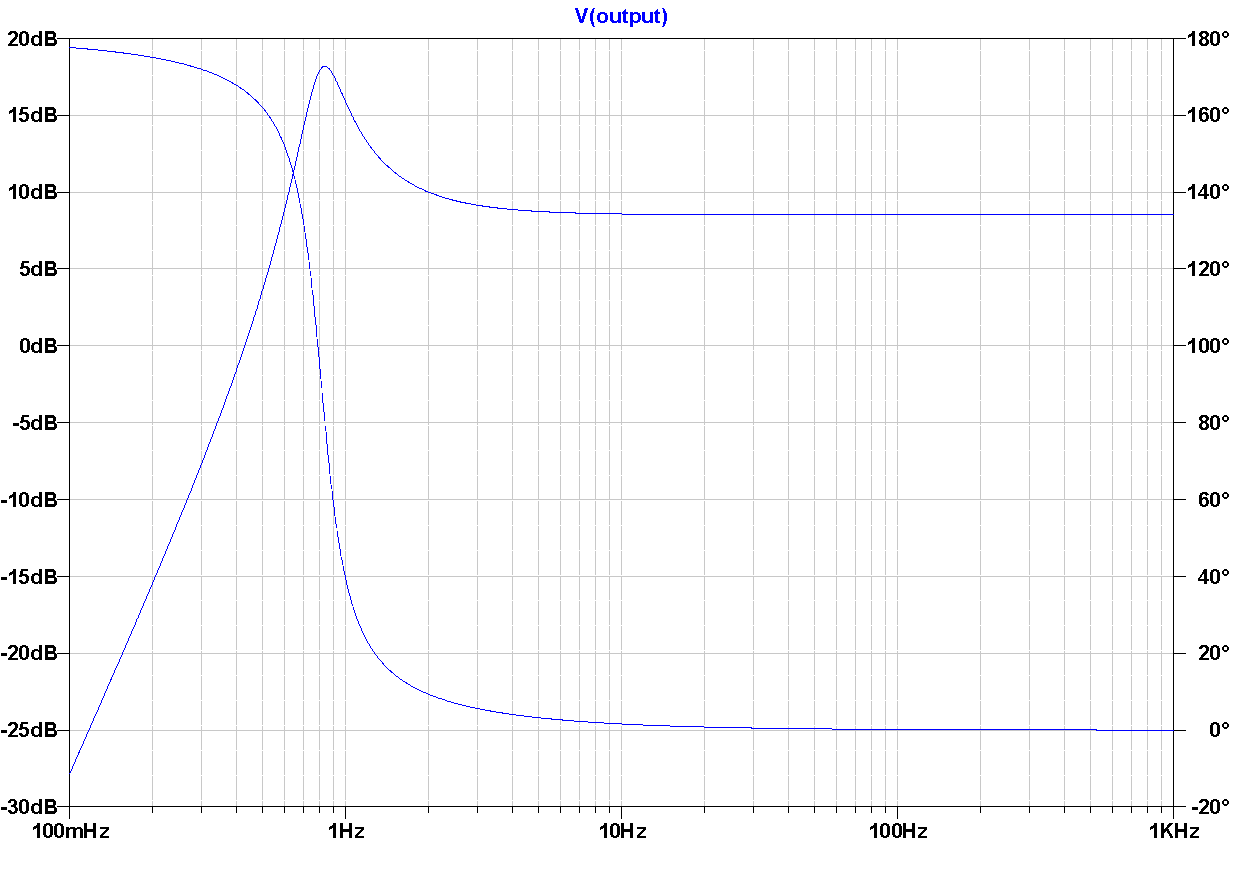
\includegraphics[width=1\linewidth]{./Figures/HPFBode.pdf}
		    \caption{} \label{subfig:HPFBodePlot}
     \end{subfigure}
     \begin{subfigure}[]{0.48\textwidth}
             \centering
  		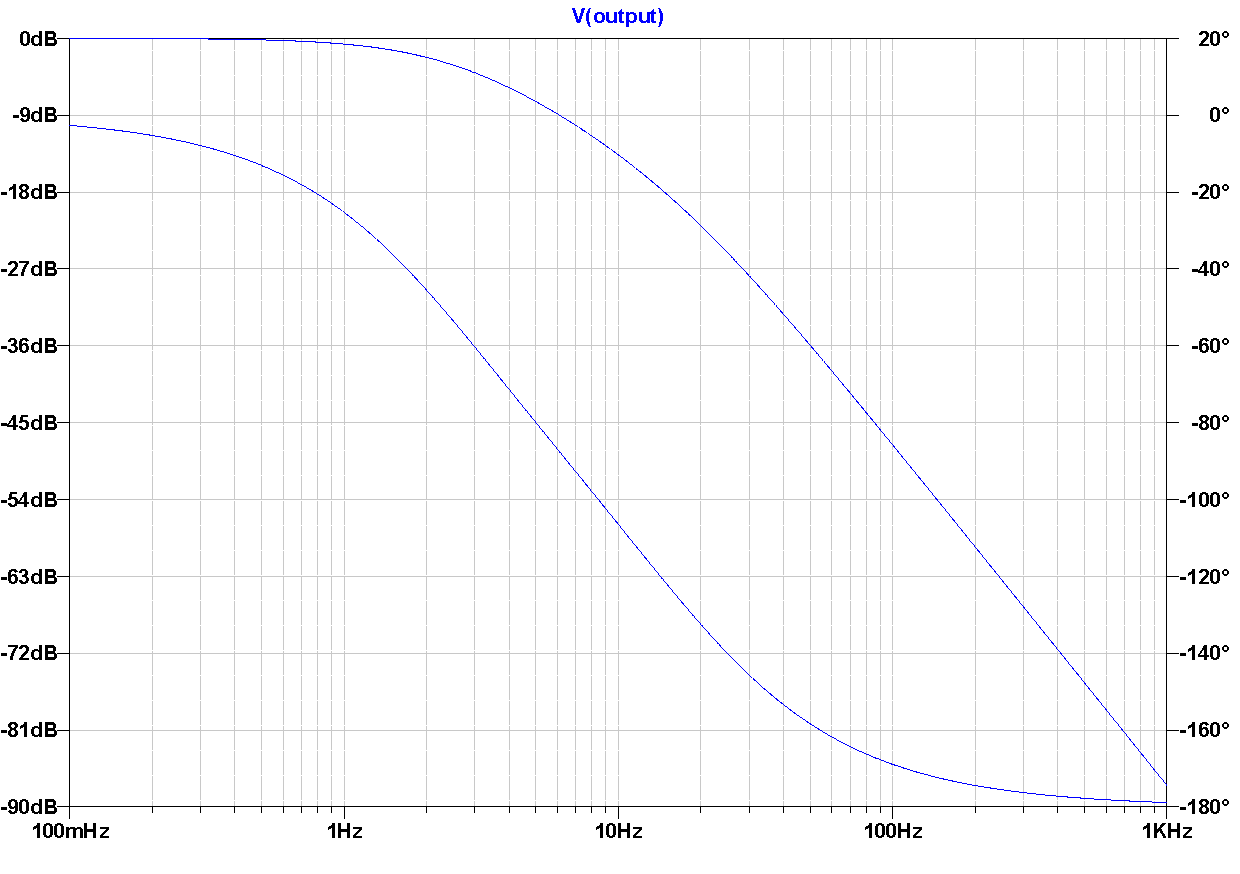
\includegraphics[width=1.0\linewidth]{./Figures/LPFBode.pdf}
		   \caption{ } \label{subfig:LPFBodePlot}
     \end{subfigure}
    \begin{subfigure}[]{0.35\textwidth}
              \centering
  		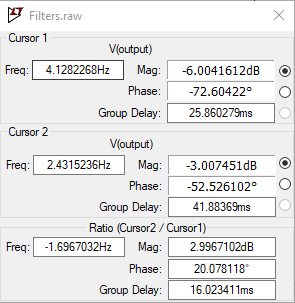
\includegraphics[width=1\linewidth]{./Figures/LPFBodeCursor.png}
		    \caption{} \label{subfig:LPFCursor}
     \end{subfigure}
    \begin{subfigure}[]{0.62\textwidth}
              \centering
  		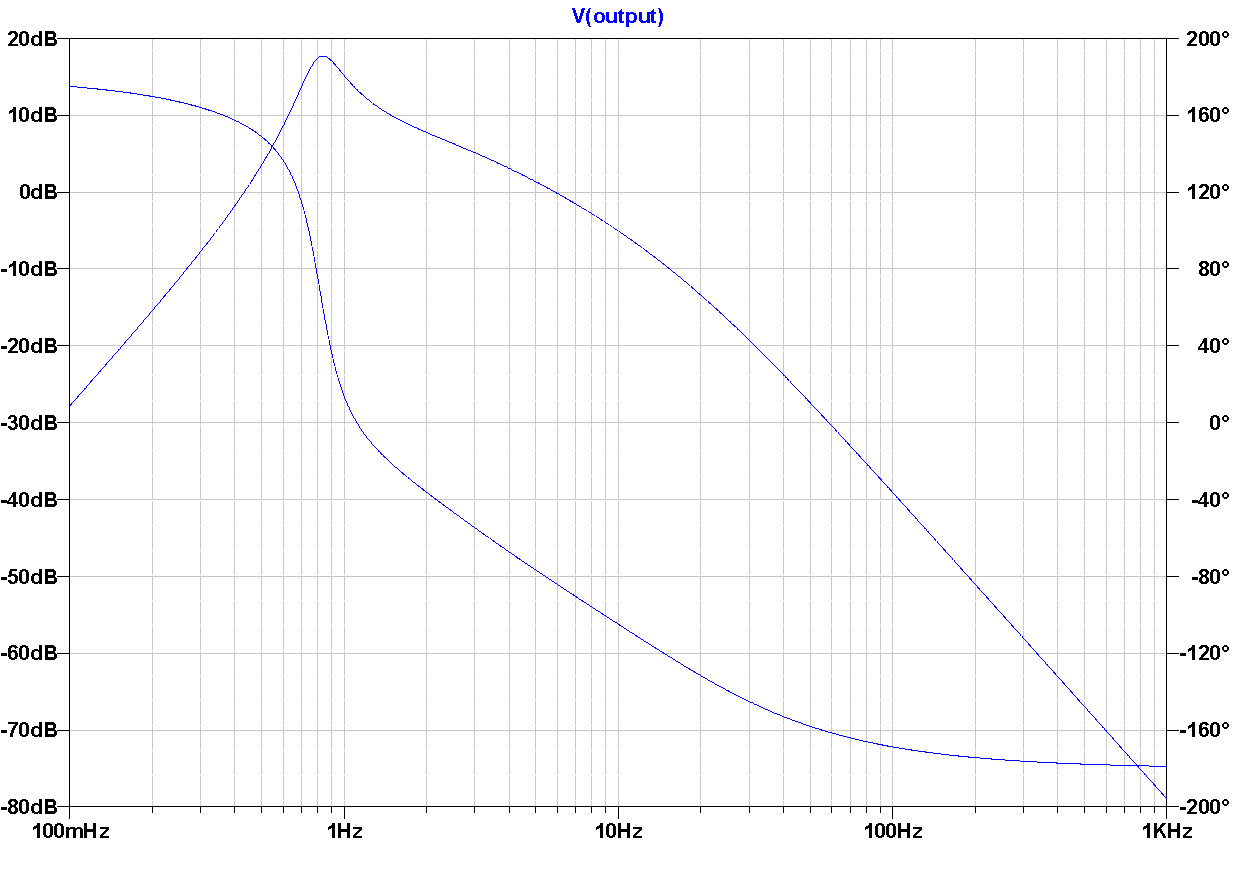
\includegraphics[width=1\linewidth]{./Figures/HPFLPFBode.pdf}
		    \caption{} \label{subfig:BPF}
     \end{subfigure}
  \caption[Bode plots of filter stages]{Bode plots of filter stages. (a) HPF Sallen Key bode Plot (b) LPF Passsive Bode Plot (c) LPF Bode plot cursors (d) Combined stages bode plot}
    \label{fig:filter_results}
 \end{figure}
 
 \begin{table}[H]
        \centering
        \footnotesize
        \caption{Table of current usage.}
         \begin{tabular}{cc@{\qquad}rrrrr}
          \toprule
             Test Frequency & Current through $R_{sense}$ \\
             $[BPM]$ & $[\SI{}{\milli\ampere}]$ \\
          \midrule
             60 & -12.4942\\
            %  90 & -12.4942\\
            %  120 & -12.4942\\
             150 & -12.4942\\
          
          \bottomrule
          Average & -12.4942
        \end{tabular}
     \label{tab:current results}
\end{table}
 
 \begin{figure}[ht]
 \footnotesize
 \centering
    % \begin{subfigure}[]{0.55\textwidth}
    %           \centering
  		% 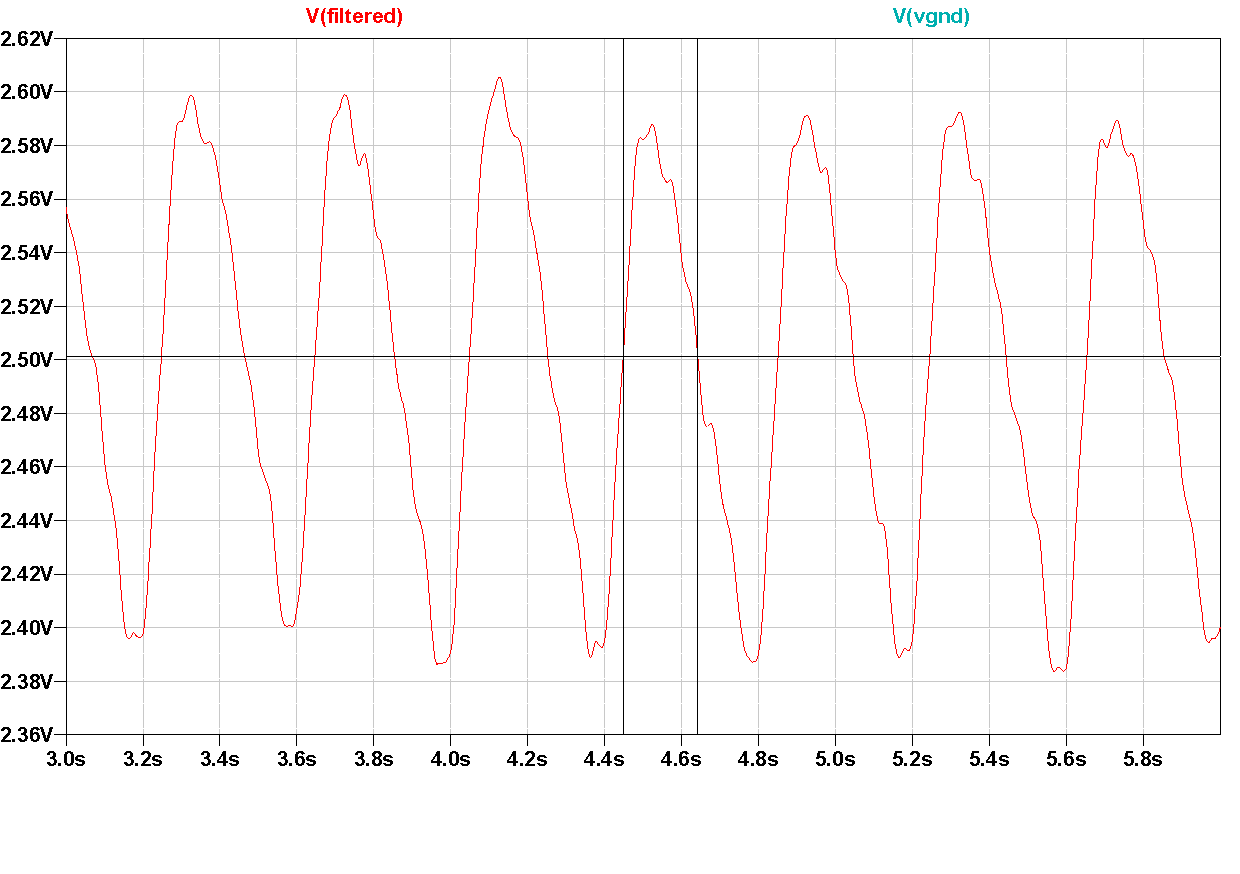
\includegraphics[width=1\linewidth]{./Figures/ThresholdResult.pdf}
		  %  \caption{} \label{subfig:Threshold}
    %  \end{subfigure}

    \begin{subfigure}[]{0.48\textwidth}
              \centering
  		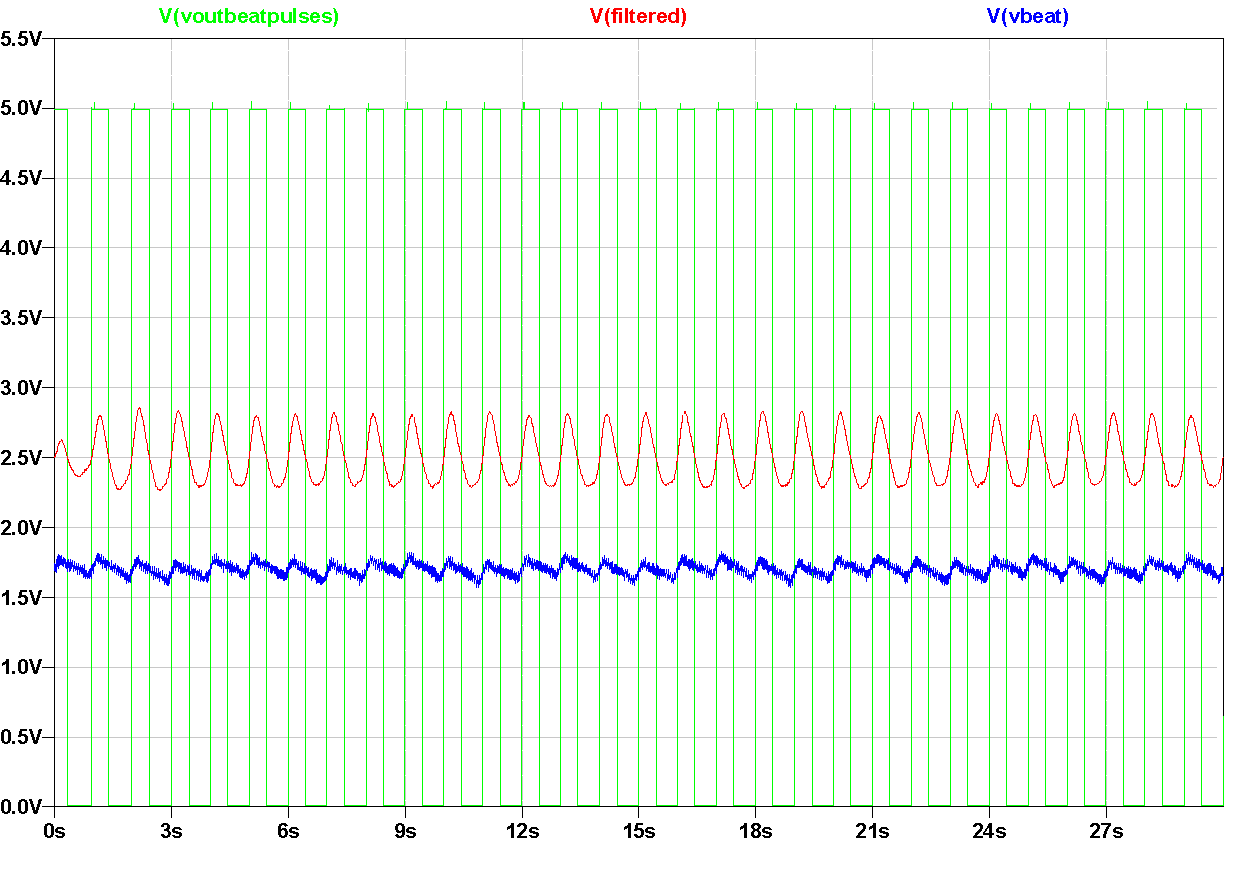
\includegraphics[width=1\linewidth]{./Figures/60BPM.pdf}
		    \caption{} \label{subfig:Pulse60}
     \end{subfigure}
     \begin{subfigure}[]{0.48\textwidth}
              \centering
  		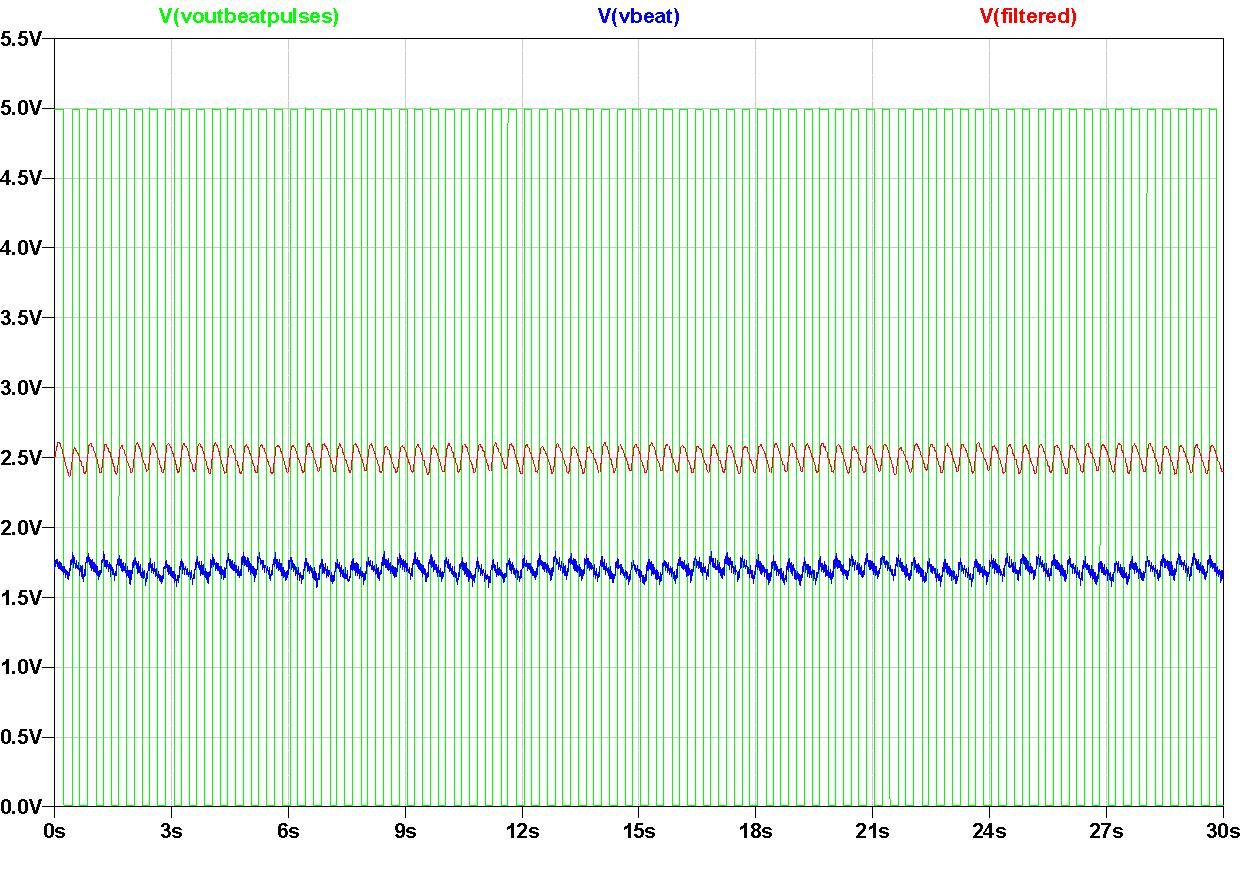
\includegraphics[width=1\linewidth]{./Figures/150BPM.pdf}
		    \caption{} \label{subfig:Pulse150}
     \end{subfigure}
    \begin{subfigure}[]{0.4\textwidth}
              \centering
  		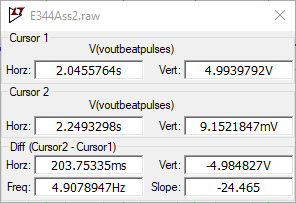
\includegraphics[width=1\linewidth]{./Figures/150BPM Pulse.png}
		    \caption{} \label{subfig:Pulse Duration}
     \end{subfigure}
     \begin{subfigure}[]{0.4\textwidth}
             \centering
  		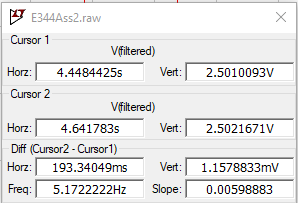
\includegraphics[width=1.0\linewidth]{./Figures/ThresholdResult.png}
		   \caption{ } \label{subfig:ThreshCursor}
     \end{subfigure}
  \caption[Thresholding \& Pulse Results]{(a) \SI{60}{BPM} signal with pulse output (b)\SI{150}{BPM} signal with pulse output (c) Cursor position for pulse duration in fig. \ref{subfig:Pulse150} (d) Cursor position for threshold values}
    \label{fig:thresholdPulse}
 \end{figure}


% In this section, you want to demonstrate, by means of referring to simulation results, using the designed circuit, how your circuit behaves as you designed it in Section \ref{sec:heartDesign}. Present and report on your simulated results in Figure \ref{fig:simulation_results_box}. Be absolutely sure that the text and information in your report are readable. 

% You can use screengrabs or photos of the oscilloscope, or download the CSVs and plot them as PDFs using Matlab, Excel or similar. 
% You can also use tables, example of which are presented in Tables \ref{tab:table1} and \ref{tab:table2}.


% \begin{table}
%         \centering
%         \footnotesize
%         \caption{Example of a simple table.}
%          \begin{tabular}{c@{\qquad}rrrr}
%           \toprule
%              & 2017 & 2018 & $\Delta_{Abs}$ & $\Delta_{DiD}$\\
%           \midrule
%           A & 9,868      & 10,399 & +5 & -11\\
%           B & 10,191     & 10,590 & +4 & -12\\
%           \bottomrule
%         \end{tabular}
%      \label{tab:table1}
% \end{table}


% \begin{table}
%          \centering
%         \footnotesize
%         \caption{Example of another table.}

%          \begin{tabular}{c@{\qquad}rrrr}
%           \toprule
%           \multirow{2}{*}{\raisebox{-\heavyrulewidth}{Schools }} & \multicolumn{2}{c}{Total energy used}& \multicolumn{2}{c}{Change}\\
%           \cmidrule{2-5}
%             & 2017 & 2018 & $\Delta_{Abs}$ & $\Delta_{DiD}$\\
%             & [kWh] & [kWh] & [\%] & [\%] \\
%           \midrule
%           A & 9,868      & 10,399 & +5 & -11\\
%           B & 10,191     & 10,590 & +4 & -12\\
%           \bottomrule
%         \end{tabular}
%      \label{tab:table2}
% \end{table}


%**********************************************
\section{Summary}\label{sec:temp_summary}
%**********************************************
The circuit performed as expected. The pulse duration for the shortest wavelength still exceeds \SI{150}{\milli\second} and the comparator pushes the signal to reach \numrange{5}{0} \si{\volt} at its highest and lowest. Small deviations in amplitude and in DC offset is also limited which ensures the signal is stable. The circuit is limited to only work efficiently between the ranges of \numrange{50}{150} BPM, as any BPM lower or higher might be filtered out. One must keep in mind that the circuit is only accurate after the \SI{1}{\second} at \SI{50}{BPM} as the capacitors need to be charged.



